\section{Sekvenční Vložení (Sequential Insertion)}
\subsection{Provedení nad automatem}
Vzhledem k faktu, že tato operace je podobná operaci shuffle, můžeme nad ní uvažovat velice podobně. V této operaci je však rozdíl, že musíme vložit řetězec z druhého jazyka nerozdělený. Nejlépe ukážeme na příkladu: 

Mějme dva jazyky $K(M)=\{CD\}$ a $L(N)=\{AA, BB\}$ a automaty kterými jsou definovány.(\ref{imgExample:insertionTeory})
\begin{figure}[H]
\centering
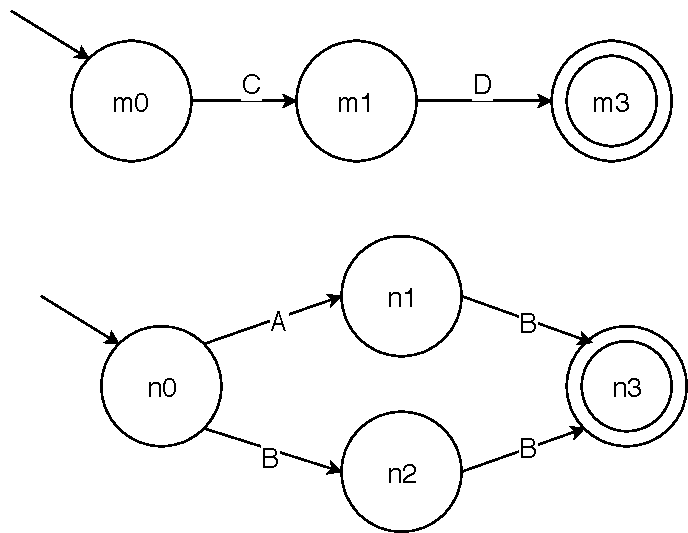
\includegraphics[width=0.7\textwidth]{obrazky-figures/IsertionPriklad.pdf}
\label{imgExample:insertionTeory}
\caption{Příklad automatů pro Sequential Insertion}
\end{figure}

Nyní nad těmito jazyky budeme chtít provést sekvenční vložení $N$ do $M$, tedy \\
$SequentialInsertion(M,N)$. Zde je si potřeba uvědomit, že můžeme provést kartézský součin k tomu abychom sledovali ve kterém jsme právě automatu. Pro jednodušší pochopení si
představme, že automat $M$ je osa $X$ a automat $N$ je osa $Y$. Sekvenční vložení nám pak říká, že musíme řetězec přijímaný automatem $N$ můžeme vložit kamkoliv do řetězce přijímaného automatem $M$. Tedy se můžeme pohybovat přechody po ose $X$
libovolně, ale ve chvíli, kdy se přesuneme po ose $Y$, musíme po této ose dojít až na konec řetězce přijímaného automatem $N$. (viz. \ref{imgExample:insertionTeoryRes})

\begin{figure}[H]
\centering
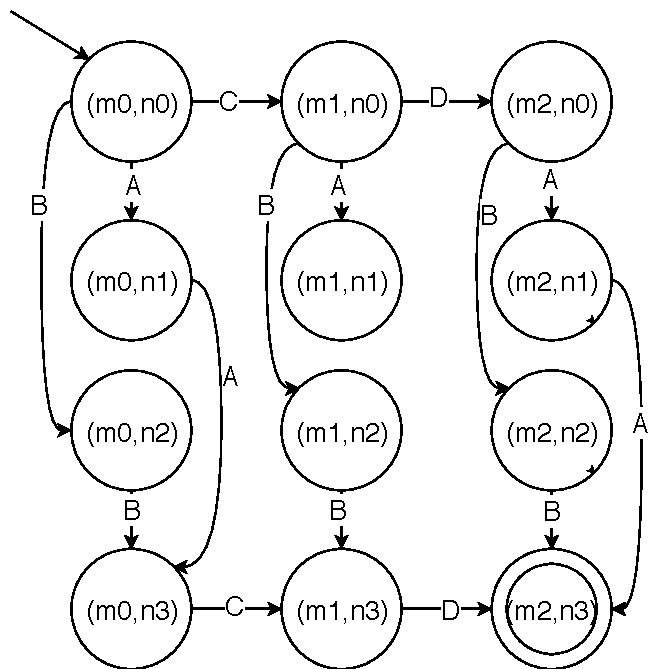
\includegraphics[width=0.7\textwidth]{obrazky-figures/IsertionPrikladResult.pdf}
\label{imgExample:insertionTeoryRes}
\caption{Výsledek po použití operace Sequential Insertion}
\end{figure}



Tento příklad si můžeme zobecnit následujícím způsobem, mějme dva automaty :

$M=\{Q_{M}, \Sigma_{M}, R_{M},s_{M}, F_{M}\}$ a $N=\{Q_{N}, \Sigma_{N}, R_{N},s_{N}, F_{N}\} $

Sekvenční vložení N do M provedeme následovně:
\begin{equation}
\label{eqA:Insertion}
\begin{split}
    Insertion(M,N) = \{ &\\
           &Q = Q_{M} \times Q_{N},\\
    &  \Sigma = \Sigma_{M} \cup \Sigma_{N} \\
    & \delta = \{ (q_{M},q_{N})\alpha \longrightarrow \left\{\begin{matrix}
 (q_{M}\alpha, q_{N})& if & q_{N}=s \vee q_N \in F_{N}\\ 
 (q_{M}, q_{N}\alpha)& else & 
\end{matrix}\right.;\\
    &\tab q_{M} \in Q_{M} \land q_{N} \in Q_{N} \land \alpha \in \Sigma\\
    &\tab\}, \\
    & s = (s_{M}, s_{N}), \\
    & F = F_{M} \times F_{N} \\
    \}&
\end{split}
\end{equation}


\subsection{Implementace}
Pravidla se vytváří dle výše uvedeného automatu, obdobně jako tomu bylo v ukázce \ref{example:shuffle}
(\textit{src/operations/sequentialInsertionFA.js})
% \begin{figure}[h]
% \centering
% \includegraphics[width=0.7\textwidth]{obrazky-figures/intersectionExample.png}
% \label{imgExample:intersection}
% \caption[]
%     {\tabular[t]{@{}l@{}}Ukázka implementace operace Intersection \\ $src/operations/intersectionFA.js$\endtabular}
% \end{figure}
